\documentclass[12pt]{article}
\usepackage[top=1in,left=1in, right = 1in, footskip=1in]{geometry}

\usepackage{graphicx}
%\usepackage{adjustbox}

\newcommand{\comment}{\showcomment}
%% \newcommand{\comment}{\nocomment}

\newcommand{\showcomment}[3]{\textcolor{#1}{\textbf{[#2: }\textsl{#3}\textbf{]}}}
\newcommand{\nocomment}[3]{}

\newcommand{\jd}[1]{\comment{cyan}{JD}{#1}}
\newcommand{\swp}[1]{\comment{magenta}{SWP}{#1}}

\newcommand{\eref}[1]{Eq.~\ref{eq:#1}}
\newcommand{\fref}[1]{Fig.~\ref{fig:#1}}
\newcommand{\Fref}[1]{Fig.~\ref{fig:#1}}
\newcommand{\sref}[1]{Sec.~\ref{#1}}
\newcommand{\frange}[2]{Fig.~\ref{fig:#1}--\ref{fig:#2}}
\newcommand{\tref}[1]{Table~\ref{tab:#1}}
\newcommand{\tlab}[1]{\label{tab:#1}}
\newcommand{\seminar}{SE\mbox{$^m$}I\mbox{$^n$}R}

\usepackage{amsthm}
\usepackage{amsmath}
\usepackage{amssymb}
\usepackage{amsfonts}

% \usepackage{lineno}
% \linenumbers

\usepackage[pdfencoding=auto, psdextra]{hyperref}

\usepackage{natbib}
\bibliographystyle{chicago}
\date{\today}

\usepackage{xspace}
\newcommand*{\ie}{i.e.\@\xspace}

\usepackage{color}

\newcommand{\Rx}[1]{\ensuremath{{\mathcal R}_{#1}}} 
\newcommand{\Ro}{\Rx{0}}
\newcommand{\Rc}{\Rx{c}}
\newcommand{\RR}{\ensuremath{{\mathcal R}}}
\newcommand{\Rhat}{\ensuremath{{\hat\RR}}}
\newcommand{\tsub}[2]{#1_{{\textrm{\tiny #2}}}}

\begin{document}

\begin{flushleft}{
	\Large
	\textbf\newline{
		Unraveling the paradox between generation and serial intervals: applications to COVID-19 pandemic
	}
}
\end{flushleft}

\section*{Abstract}

\pagebreak

\section{Introduction}

Since the emergence of the novel coronavirus disease (COVID-19), a significant amount of research has focused on estimating its reproduction number $\mathcal R$ \citep{majumder2020early}.
The reproduction number is defined as the average number of secondary cases caused by a primary case;
the corresponding reproduction number in a fully susceptible population --- referred to as the basic reproduction number $\mathcal R_0$ --- allows us to predict the extent to which a disease will spread in the population and the amount of intervention to prevent an outbreak \citep{anderson1991infectious}.
Since reproduction numbers cannot be measured directly, particularly during the outset of an outbreak, it is often estimated from the observed exponential growth rate using generation- and serial-interval distributions (e.g., \cite{du2020serial, jung2020real, li2020early, zhao2020preliminary}).

The generation interval is defined as the time between when an individual (infector) is infected and when an individual infects another person (infectee);
the generation-interval distributions plays a key role in shaping the relationship between the exponential growth rate $r$ and the reproduction number $\mathcal R$ \citep{wallinga2007generation}.
Similarly, the serial interval is defined as the time between when an infector and an infectee become \emph{symptomatic} \citep{svensson2007note}.
While serial intervals are similar to generation intervals, previous studies have noted that, in many contexts, serial intervals are expected to have larger variances than generation intervals but have the same mean \citep{svensson2007note,klinkenberg2011correlation,champredon2018equivalence};
some studies further suggested that using serial intervals can give different estimates of $\mathcal R$ \citep{britton2019estimation}.
Even these distributions were clearly distinguished over a decade ago \citep{svensson2007note}, 
the need for a better conceptual and theoretical framework for understanding their differences is becoming clearer as the COVID-19 pandemic unfolds:
Researchers continue to rely on both generation and serial intervals to estimate $\mathcal R$ for COVID-19 without making a clear distinction.

One important source of confusion comes down to an apparent paradox.
When the epidemic is growing exponentially, the spread of infection can be characterized as a ``renewal process'' based on previous incidence of infection, the associated generation-interval distribution, and the average infectiousness of an infected individual.
This renewal formulation allows us to link the exponential growth rate of an epidemic $r$ with its reproduction number $\mathcal R$ \citep{wallinga2007generation}.
Likewise, we should be able to describe the renewal process of symptomatic cases using the serial-interval distribution.
Therefore, both generation- and serial-interval distributions should give us identical estimates of  $\mathcal R$ based the observed epidemic growth rate $r$.
In contexts where the distributions are expected to be different, current theory has no explanation for how they might link $r$ to \Rx\ in the same way.

Here, we provide an answer to this paradox, by showing that the relevant interval for the renewal framework is what is called the ``forward'' interval, and that the forward serial (but not generation) interval is affected by the rate of growth $r$ during the exponential-growth phase.
We develop a new framework for understanding serial intervals and show that the forward serial-interval distribution gives the correct value of $\mathcal R$.
%\jd{Come back to this. Not just over time, right?} \swp{What do you mean? Everything is about time here... you haven't read the results section so maybe that's why?}
However, using inaccurately defined serial intervals or failing to account for changes in the observed serial-interval distributions over the course of an epidemic can bias the estimate of $\mathcal R$.
We apply our framework to serial intervals of COVID-19 and lay out several principles to consider in using information about serial intervals and other epidemiological time delays in the analysis of the ongoing pandemic.

\section{Methods}

\subsection{Backward and forward delay distributions}

We first begin by describing a general framework for characterizing a distribution of time delays between two epidemiological events;
these events can be defined either within an infected individual (e.g., infection and symptom onset of an individual, the incubation period) or between infected individuals (e.g., symptom onsets of an infector and an infectee, the serial interval).
We can further divide these events into \emph{primary} and \emph{secondary} events.
When we measure an epidemiological time delay within an infected individual (e.g., the incubation period), the primary event is the event that always or usually occurs before the secondary event ---
most epidemiological events that can be observed within an individual have clear direction (e.g., infection and onset of symptoms) but some may not (e.g., onset of infectiousness and onset of symptoms).
% \jd{Rethink, or else rethink ``any'' above: the ``hidden'' time (my term) is the time between onset of infectiousness and onset of symptoms; it is within, but can be positive or negative. I'm not saying we should use it here\ldots}
When we measure an epidemiological time delay between infected individuals (e.g., the serial interval), 
the primary and secondary events are defined in terms of the direction of transmission:
The primary event refers to the event that occurs within an infector and does not necessarily occur before the secondary event.

We model time delays between a primary and a secondary event from a cohort perspective.
A primary cohort consists of \emph{all} individuals whose primary event occurred at a given time; 
a secondary cohort is defined similarly based on the secondary events.
For example, when we are measuring serial intervals, a primary cohort $\pi$ consists of all infectors who became symptomatic at time $\pi$.
Then, for each primary cohort $\pi$, we can define the expected time distribution between primary and secondary events.
We refer to this distribution as the forward delay distribution and denote it as $f_\pi(\tau)$.
%% The forward delay distributions can vary across primary cohorts.
%% \jd already implied, and may block the flow

Likewise, we define the backward delay distribution $b_\delta(\tau)$ for a secondary cohort $\delta$:
The backward delay distribution describes the time delays between a primary and secondary host given that the secondary event occurred at time $\delta$.
Since both forward and backward perspectives provide valid ways of measuring time delays, we can express the total density of primary and secondary events occurring at time $\pi$ and $\delta$, respectively, using both forward and backward delay distributions:
\begin{equation}
P(\pi) f_\pi(\delta-\pi) = D(\delta) b_\delta(\delta-\pi),
\end{equation}
where $P$ and $D$ represent the sizes of primary and secondary cohorts, respectively.
Substituting $\tau = \delta - \pi$, it follows that:
\begin{equation}
b_\delta(\tau) = \frac{P(\delta-\tau) f_{\delta-\tau}(\tau)}{D(\delta)}
\end{equation}
Therefore, the backward delay distribution depends on the changes in primary cohort size $P$ (therefore incidence of infection) as well as changes in the forward delay distribution.
These ideas apply to all epidemiological delay distributions and generalize the work by \citep{champredon2015intrinsic} who compared forward and backward generation-interval distributions to describe the realized generation intervals from the perspective of an infector and an infectee, respectively.

\subsection{Realized serial interval distributions}

The serial interval is defined as the time between when an infector becomes symptomatic and when and infectee becomes symptomatic.
Serial intervals $\tau$ have been typically written in the form of:
\begin{equation}
\tau = - x_0 + \sigma + x_1
\end{equation}
where $x_0$ and $x_1$ represent the realized time from infection to symptom onset of an infector and an infectee, respectively, and $\sigma$ represents the realized generation interval.
Previous studies have often assumed that $x_0$ and $x_1$ follow the same distributions and concluded that the serial and generation intervals have the same mean \citep{svensson2007note,klinkenberg2011correlation,champredon2018equivalence, britton2019estimation}.
% \jd{I would drop the last clause. I still argue that this is true for intrinsic SIs, and we don't want to get into that here. You can just keep rolling forward at this point.}

\begin{figure}[!th]
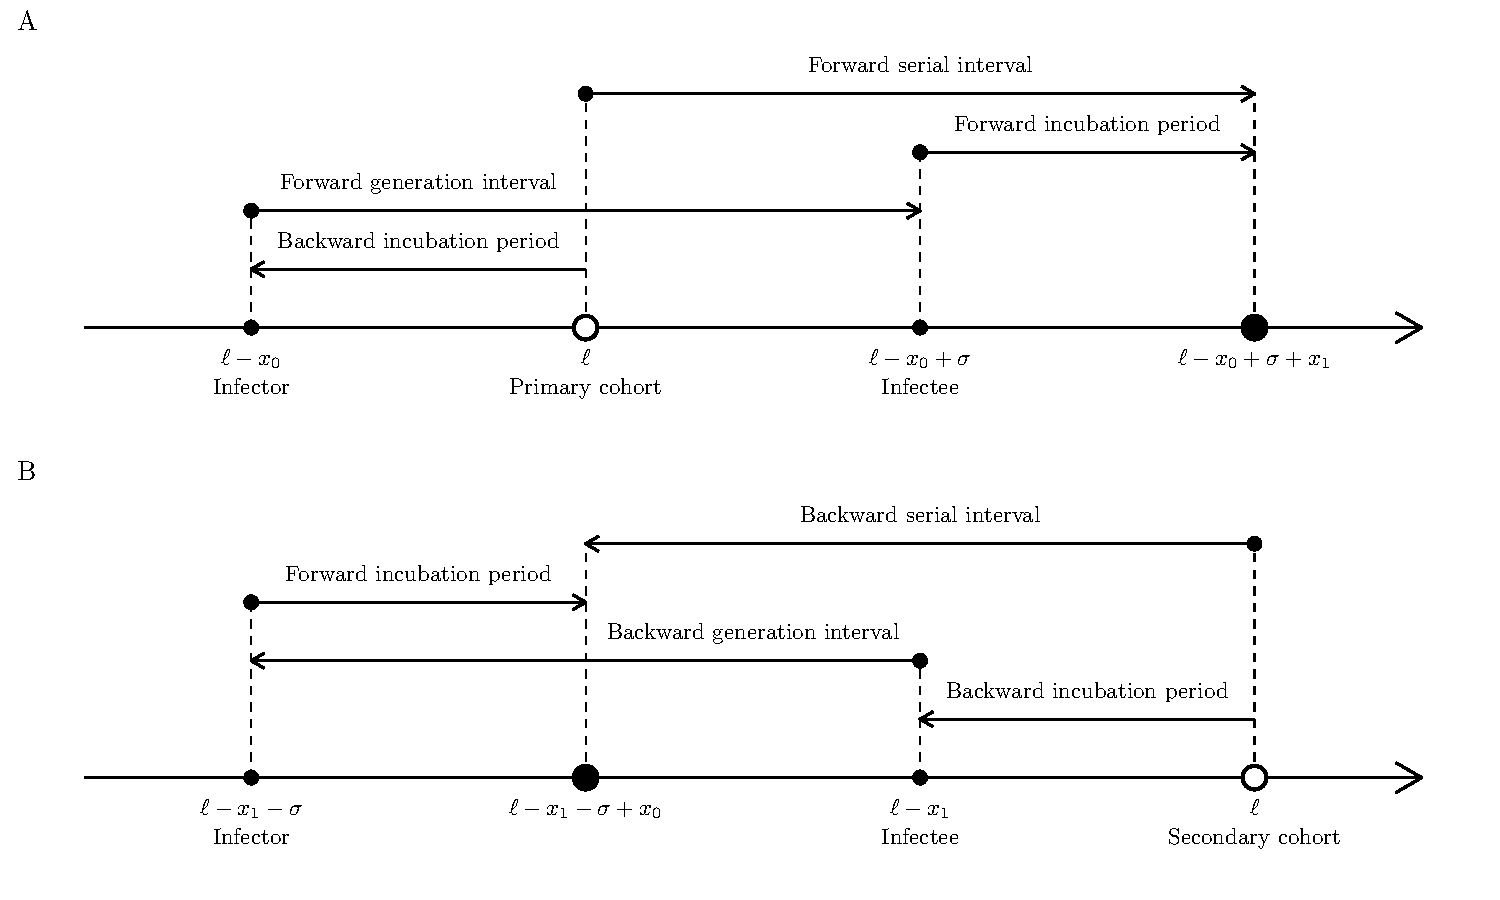
\includegraphics[width=\textwidth]{serial_guide.pdf}
\caption{
\textbf{Illustration of forward and backward serial intervals.}
A. The forward serial interval for a primary cohort $\ell$ (i.e., an infector who became symptomatic at time $\ell$).
In this case, $x_0$ represents the backward incubation period of the infector;
$\sigma$ represents the forward generation interval;
and $x_1$ represents the forward incubation period of the infectee.
B. The backward serial interval for a secondary cohort $\ell$ (i.e., an infectee who became symptomatic at time $\ell$).
In this case, $x_0$ represents the forward incubation period of the infector;
$\sigma$ represents the backward generation interval;
and $x_1$ represents the backward incubation period of the infectee.
}
\label{fig:diagram}
\end{figure}

The cohort-based framework allows us to understand the distribution of serial intervals we expect to observe when incidence is changing.
Given that an infector became symptomatic at time $\pi$, we first go backward in time by asking when the infector was infected, and then go forward in time by asking first when the infectee was infected and then when the infectee became symptomatic;
this defines the forward serial interval.
In \fref{diagram}A, we see that $x_0$ represents the backward incubation period of the infector who became symptomatic at time $\pi$;
$\sigma$ represents the forward generation interval of the infector who came infected at time $\pi - x_0$;
and $x_1$ represents the forward incubation period for the infectees who became infected at time $\pi - x_0 + \sigma$.

Likewise, we can define the backward serial interval distribution for a secondary cohort $\delta$ (\fref{diagram}B).
Given that an infectee became symptomatic at time $\delta$, we have to first go backward in time by asking when the infectee became infected and when the infector became infected; 
then, we have to go forward in time by asking when the infector became symptomatic.
In this case, $x_1$ represents the backward incubation period of the infectee who became symptomatic at time $\delta$;
$\sigma$ represents the backward generation interval of the infectee who became infected at time $\delta-x_1$;
and $x_0$ represents the forward incubation period of the infector who became infected at time $\delta-x_1-\sigma$.
This conceptual framework clearly demonstrates that the distributions of $x_0$, $\delta$, and $x_1$ (and therefore the distributions of serial intervals) depend on the perspective as well as time and cannot be treated statically.

In order to define forward and backward serial interval distributions, we begin by writing the total number of serial intervals between time $\pi$ (when the infector developed symptoms) and $\delta$ (when the infectee developed symptoms), which can be expressed as an integral over all of the possibilities for the infection times of the infector $\alpha_1$ and the infectee $\alpha_2$:
\begin{equation}
T(\pi,\delta) = \int_{-\infty}^{\pi} \int_{\alpha_1}^{\delta} \mathcal R_c (\alpha_1) i(\alpha_1) h_{\alpha_1}(\pi-\alpha_1, \alpha_2 - \alpha_1) k_{\alpha_2}(\delta - \alpha_2) \mathrm{d}\alpha_2\,\mathrm{d}\alpha_1,
\end{equation}
where $\mathcal R_c(\alpha_1)$ is the case reproduction number (i.e., the average number of secondary cases caused by a primary case infected at time $\alpha_1$, \cite{fraser2007estimating}), $i(\alpha_1)$ is incidence, $h_{\alpha_1}(\pi-\alpha_1, \alpha_2 - \alpha_1)$ is the joint probability distribution describing the forward incubation period $\pi-\alpha_1$ and forward generation interval $\alpha_2 - \alpha_1$ of an individual infected at time $\alpha_1$ (in this case, the infector), and $k_{\alpha_2}(\delta-\alpha_2)$ describes the marginal probability distribution of $h_{\alpha_2}$ describing the forward incubation period $\delta-\alpha_2$ of an individual infected at time $\alpha_2$ (in this case, the infectee). 
Then, the forward serial-interval distribution is proportional to $T(\pi, \pi+\tau)$. Substituting $x=\pi-\alpha_1$ and $\sigma=\alpha_2-\alpha_1$, we have:
\begin{equation}
f_\pi(\tau) \propto \int_{0}^{\infty} \int_{0}^{x+\tau} \mathcal R_c (\pi-x) i(\pi-x) h_{\pi-x}(x, \sigma) k_{\pi-x+\sigma}(x-\sigma+\tau) \mathrm{d}\sigma\,\mathrm{d}x
\end{equation}
Likewise, the backward serial-interval distribution is proportional to $T(\delta-\tau, \delta)$. 
This time, we substitute $x=\delta-\alpha_2$ and $\sigma=\alpha_2-\alpha_1$ to get:
\begin{equation}
b_\delta(\tau) \propto \int_{0}^{\infty} \int_{\max(0, \tau-x)}^{\infty} \mathcal R_c (\delta-x-\sigma) i(\delta-x-\sigma) h_{\delta-x-\sigma}(x+\sigma-\tau, \sigma) k_{\delta-x}(x) \mathrm{d}\sigma\,\mathrm{d}x.
\end{equation}

%Hereafter, we assume that the forward incubation period distributions does not vary across cohorts over the course of an epidemic, as they represent the natural history of a disease, and use $k$ without subscript instead:
%\begin{equation}
%k(x) = \int_0^\infty h_\pi(x, \sigma) \mathrm{d}\sigma.
%\end{equation}

\subsection{Epidemic model}

We validate the theory by applying it to a specific example of an epidemic model. 
We model disease spread with a renewal-equation model \citep{heesterbeek1996concept, diekmann2000mathematical, roberts2004modelling, aldis2005integral, roberts2007model, champredon2018equivalence}.
Ignoring births and deaths, changes in the proportion of susceptible individuals $S(t)$ and incidence of infection $i(t)$ can be written as:
\begin{equation}
\begin{aligned}
\frac{\mathrm{d}S}{\mathrm{d}t} &= - i(t)\\
i(t) &= \mathcal R_0 S(t) \int_0^\infty i(t-\tau) g(\tau) \mathrm{d}\tau,
\end{aligned}
\label{eq:renewal}
\end{equation}
where $\mathcal R_0$ is the basic reproduction number, and $g(\tau)$ is the intrinsic generation-interval distribution (i.e., the forward generation-interval distribution of a primary case in a fully susceptible population; \cite{champredon2015intrinsic}).
Then, the forward generation-interval for a primary cohort $\ell$ follows \citep{champredon2015intrinsic}:
\begin{equation}
g_\ell (\tau) \propto g(\tau) S(\ell + \tau),
\end{equation}
which allows us to separate the joint probability distribution $h_\ell$ of the forward incubation period and the forward generation-interval distribution as a product of the proportion of susceptible individuals $S$ and the joint probability distribution $h$ of the forward incubation period and the intrinsic generation intervals:
\begin{equation}
h_\ell (x_0, \tau) \propto h(x_0, \tau) S(\ell + \tau),
\end{equation}
which satisfies the following:
\begin{equation}
g(\tau) = \int_0^\infty h(x_0, \tau) \mathrm{d}x_0.
\end{equation}
Finally, the cohort reproduction for this model is defined as follows:
\begin{equation}
\mathcal R_c(t) = \mathcal R_0 \int_0^\infty g(\tau) S(t+\tau) \mathrm{d} \tau.
\end{equation}

\subsection{Linking $r$ and $\mathcal R$}

During the initial phase of an epidemic, the proprotion susceptible remains constant ($S(t) = S(0)$) and incidence of infection grows exponentially: $i(t)=i_0\exp(rt)$.
Then, we can estimate the reproduction number from the exponential growth rate $r$ via the Euler-Lotka equation:
\begin{equation}
\frac{1}{\mathcal R} = \int_0^\infty \exp(-r\tau) g(\tau) \mathrm{d} \tau.
\end{equation}
Like forward generation-interval distributions, 
forward serial-interval distributions describe the renewal process of symptomatic cases.
Therefore, the forward serial-interval distribution $f_{\textrm{\tiny exp}}(\tau)$ during the exponential growth phase provides the identical $r$--$\mathcal R$ link as the intrinsic generation-interval distribution:
\begin{equation}
\frac{1}{\mathcal R} = \int_{-\infty}^\infty \exp(-r\tau) f_{\textrm{\tiny exp}}(\tau) \mathrm{d} \tau,
\end{equation}
where the forward serial-interval distribution during the exponential growth phase is defined as:
\begin{equation}
f_{\textrm{\tiny exp}}(\tau) \propto \int_{0}^\infty \int_{0}^\infty \exp( -r x_0) h(x_0, \sigma) k(\tau-\sigma+x_0) \mathrm{d} x_0\, \mathrm{d}\sigma.
\end{equation}
In Appendix, we provide a mathematical proof that this relationship holds.

We note that the forward serial-interval distribution depends on the exponential growth rate $r$.
When the epidemic grows fast (high $r$), we expect the backward incubation period to be short, and therefore, the forward serial-interval distribution will generally have a larger mean than the intrinsic generation-interval distribution.
The Susceptible-Exposed-Infected-Recovered model, which assumes that incubation and exposed periods are equivalent, is a special case where the conditional forward generation-interval distribution cancels out with the backward generation-interval distribution exactly because (i) infected individuals can only transmit after symptom onset and (ii) the time between symptom onset to infection is independent of the incubation period of an infector;
in this case, the forward serial- and generation-intervals have the same distributions during the exponential growth phase.

\begin{table}[!th]
\begin{center}
\begin{tabular}{|l|l|r|}
\hline
Parameter & Values & Source\\
\hline
Mean forward incubation period & 5.5 days & \cite{lauer2020incubation} \\
SD forward incubation period & 2.4 & \cite{lauer2020incubation} \\
Mean intrinsic generation interval & 5 days & \cite{ferretti2020quantifying} \\
SD intrinsic generation interval & 2 & \cite{ferretti2020quantifying} \\
\hline
\end{tabular}
\end{center}
\caption{
\textbf{Parameter values used for simulations.}
The intrinsic generation-interval distribution is parameterized using a log-normal distribution with log mean $\mu_G=1.54$ and log standard deviation $\sigma_G=0.37$.
The forward incubation period distribution is parameterized using a log-normal distribution with log mean $\mu_I=1.62$ and log standard deviation $\sigma_I=0.42$.
The joint probability distribution is modeled using a multivariate log-normal distribution with correlations $\rho=-0.5, 0, 0.5$.
}
\end{table}

We use a simulation-based approach to compare the estimates of $\mathcal R$ based on the serial- and generation-interval distributions. 
To do so, we model the intrinsic generation-interval distribution and the incubation period using a multivariate log-normal distribution with log means $\mu_G, \mu_I$, log standard variances $\sigma_G^2, \sigma_I^2$, and correlation $\rho$;
the multivariate log-normal distribution is parameterized based on pameter estimates for COVID-19 (Table 1).
We construct forward serial intervals during the exponential growth period as follows:
\begin{equation}
S_i = -B_i + (G_i|B_i) + I_i,
\end{equation}
where the backward incubation period $B_i$ of an infector is simulated by drawing random log-normal samples $A_i$ with log mean $\mu_I$ and log variance $\sigma_I^2$ and resampling $A_i$, each weighted by the inverse of the exponential growth function $\exp(-rA_i)$;
the intrinsic generation interval conditional on the incubation period of the infector $(G_i|B_i)$ is drawn from a log-normal distribution with log mean $\mu_G + \sigma_G \rho (\log(B_i) - \mu_I)/\sigma_I$ and log variance $\sigma_G^2 (1-\rho^2)$;
the forward incubation period $I_i$ of an infectee is drawn from a log-normal distribution with log mean $\mu_I$ and log variance $\sigma_I^2$.
We then calculate the reproduction number $\mathcal R$ using the empirical estimator:
\begin{equation}
\mathcal R = \frac{1}{\frac{1}{N}\sum_{i=1}^N \exp(- r S_i)}.
\end{equation}
We compare this with an estimate of $\mathcal R$ based on naive serial-interval distribution that assumes that the backward and the forward incubation periods are identically distributed \citep{svensson2007note,klinkenberg2011correlation,champredon2018equivalence, britton2019estimation}:
\begin{equation}
{\mathcal R}_{\textrm{\tiny naive}} = \frac{1}{\frac{1}{N}\sum_{i=1}^N \exp(- r T_i)},
\end{equation}
where
\begin{equation}
T_i = -A_i + (G_i|A_i) + I_i.
\end{equation}

\section{Results}

First, we compare the estimates of the reproduction number $\mathcal R$ based on the intrinsic generation-interval distribution $g(\tau)$ and the forward serial-interval distribution during the exponential growth phase $f_{\textrm{\tiny exp}}(\tau)$.
Both distributions provide identical estimates of $\mathcal R$ regardless of the correlation $\rho$ between the incubation period distribution and the intrinsic generation-interval distribution (\fref{rR}A).
On the other hand, using naive serial-interval distributions that do not account for disease dynamics (i.e., assuming that the backward and the forward incubation period distributions are identical) underestimates $\mathcal R$;
as $r$ increases, ${\mathcal R}_{\textrm{\tiny naive}}$ saturates and eventually decreases due to negative serial intervals (\fref{rR}B).
While the forward serial intervals during the exponential growth phase can be also negative, the proportion of negative intervals are appropriately balanced because faster epidemic growth will lead to shorter backward incubation period (and therefore less negative serial intervals).

\begin{figure}[!th]
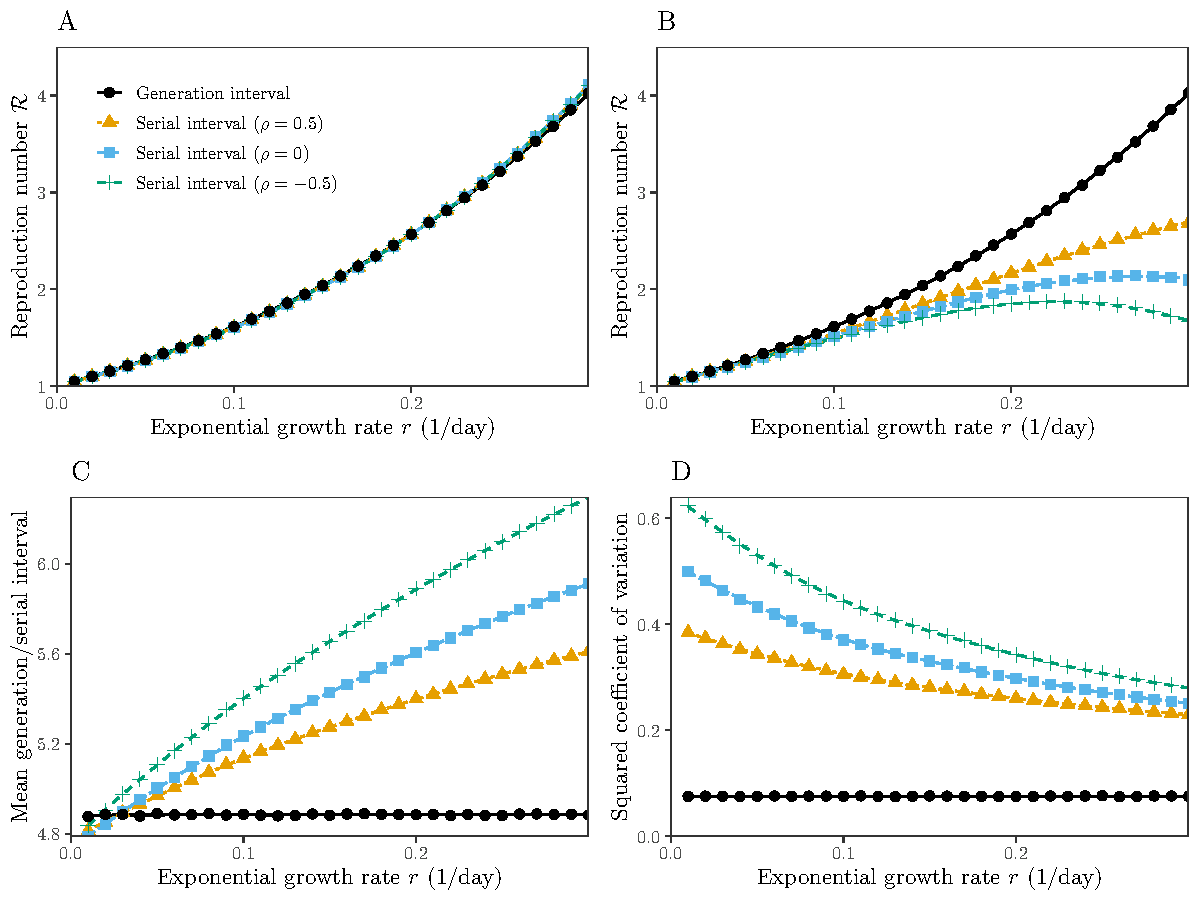
\includegraphics[width=\textwidth]{rR.pdf}
\caption{
\textbf{Estimates of the reproduction number from the exponential growth rate based on serial- and generation-interval distributions.}
A. The forward serial-interval distribution during the exponential growth phase give a correct link between the exponential growth rate $r$ and the reproduction number $\mathcal R$.
B. The serial-interval distributions that assume that the backward incubation period of an infector and the forward incubation period of an infectee are identically distributed give an incorrect link between $r$ and $\mathcal R$.
C. The mean forward serial interval during the exponential growth phase depends on $r$.
D. The squared coefficient of variation of forward serial intervals during the exponential growth phase depends on $r$.
}
\label{fig:rR}
\end{figure}

Comapring the shapes of forward serial-interval distributions and the intrinsic generation-interval distribution allow us to better understand how they are able to give identical estimates of $\mathcal R$.
In general, generation-interval distributions with higher means and less variability are expected to give higher $\mathcal R$ for a given $r$.
In this case, the forward serial intervals during the exponential growth phase have higher means (\fref{rR}C) and squared coefficients of variation (\fref{rR}D) than the intrinsic generation-interval distribution.
The effects of higher means (which increases $\mathcal R$) and higher variability (which decreases $\mathcal R$) cancel out exactly;
therefore, we estimate the same $\mathcal R$ using both serial and generation intervals.

\begin{figure}[!ht]
\begin{center}
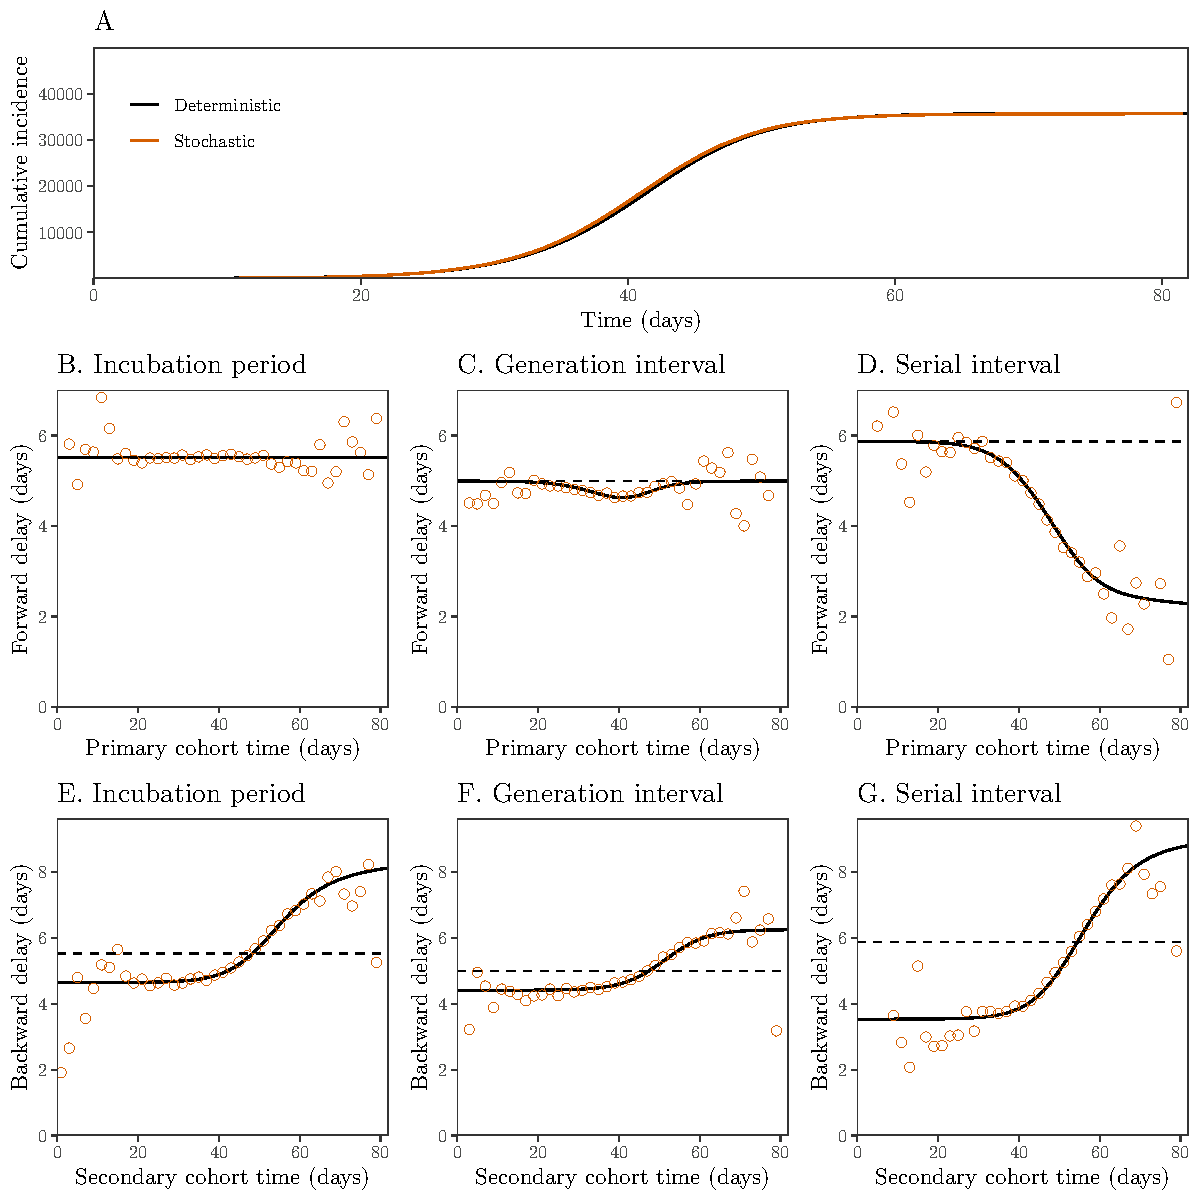
\includegraphics[width=0.95\textwidth]{forward.pdf}
\caption{
\textbf{Epidemiological dynamics and changes in mean forward and backward delay distributions.}
A. Cumulative incidence over time.
B-D. Changes in the mean forward incubation period, generation interval, and serial interval.
E-G. Changes in the mean backward incubation period, generation interval, and serial interval.
Black lines represent the results of a deterministic simulation.
Orange lines and points represent the average of 10 stochastic simulations;
cumulative incidence from the stochastic simulations in panel A are shown without averaging.
Forward incubation periods and intrinsic generation-intervals are assumed to be independent of each other: $h(x_0, \sigma) = k(x_0) g(\sigma)$.
See Table 1 for parameter values.
}
\end{center}
\label{fig:epi}
\end{figure}

\fref{epi} compares the epidemiological dynamics (A) with the mean forward (B--D) and the mean backward (E--F) delay distributions of a deterministic model based on the renewal equation (\eref{renewal}) and the corresponding stochastic realizations based on the Gillespie algorithm.
The mean forward incubation period remains constant throughout an epidemic as expected (\fref{epi}B).
The mean forward generation interval contracts as the epidemic progresses because an infected individual is less likely to infect another person as the proportion of susceptible individuals decreases (\fref{epi}C; \cite{champredon2015intrinsic}).
In contrast, the mean serial interval depends on previous incidence and therefore decreases over time (\fref{epi}D):
When incidence is increasing, symptomatic individuals are more likely to have been infected more recently (shorter backward incubation period and therefore longer forward serial interval) whereas when incidence is decreasing, symptomatic individuals are more likely to have been infected later (longer backward incubation period and therefore shorter forward serial interval).
Qualitative patterns in the changes in the mean backward delays is robust across all delay distributions because they are predominantly driven by the changes in incidence (\fref{epi}D).

\begin{figure}[!th]
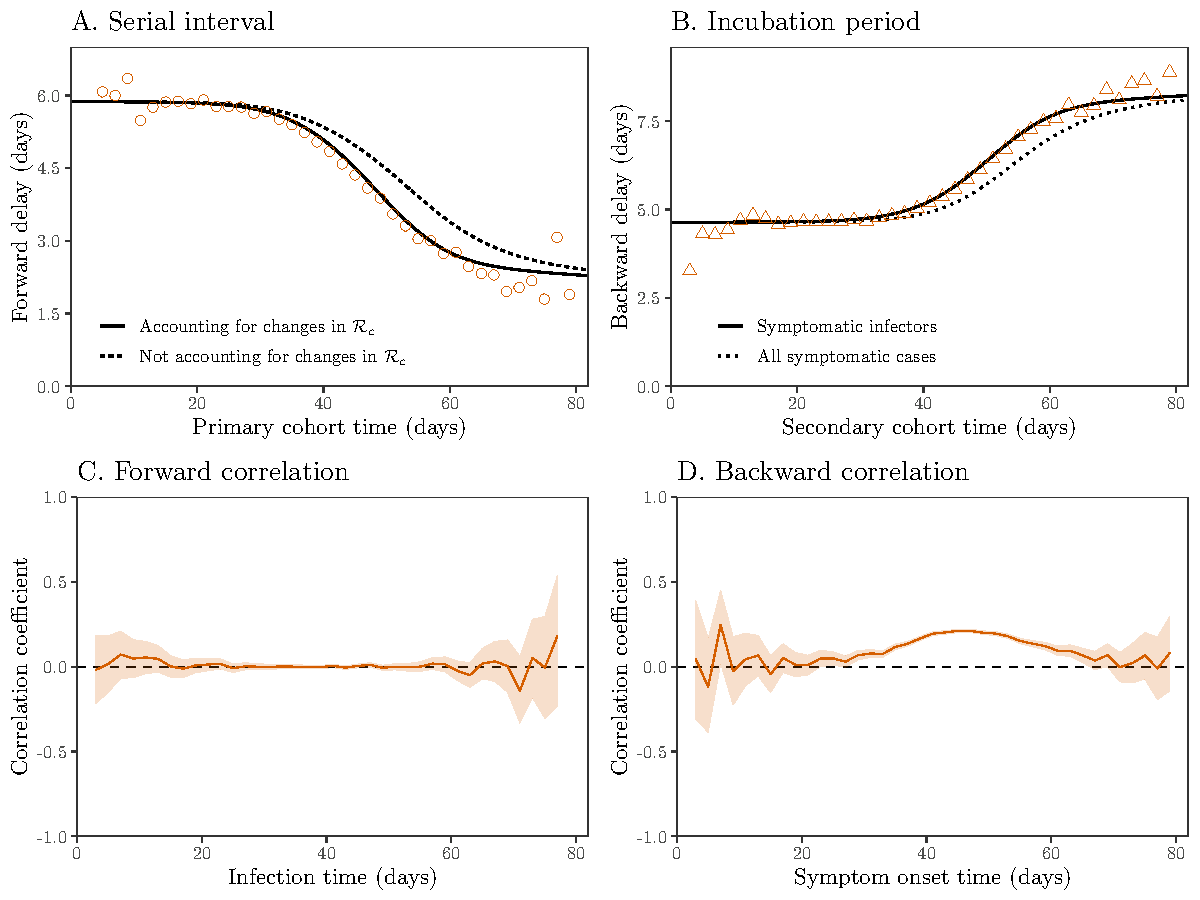
\includegraphics[width=\textwidth]{forward_tease.pdf}
\caption{
\textbf{Dynamical correlations between incubation periods and the number of secondary cases.}
A. The mean forward serial interval depends on changes in the cohort reproduction number.
B. The mean backward incubation period of infectors is higher than the mean backward incubation period of all symptomatic cases.
C. Correlation between the number of secondary cases and the incubation period for individuals who got infected within the same time preiod.
D. Correlation between the number of secondary cases and the incubation period for individuals who developed symptoms within the same time preiod.
Black lines represent the results of a deterministic simulation.
Orange lines and points represent the average of 10 stochastic simulations.
Orange ribbons represent the 95\% confidence intervals.
}
\label{fig:tease}
\end{figure}

We further tease apart factors that affect the forward serial interval distribution.
\fref{tease}A compares the mean forward serial interval calculated from a deterministic model and its corresponding stochastic simulations;
failing to account for changes in $\mathcal R_c$ in \eref{forward} overestimates the mean forward serial interval.
A key distinction that needs to be made is that the forward serial-interval distributions depend on the backward incubation period of symptomatic infectors (i.e., those who were able to successfully spread the disease to another person), rather than the incubation period of all symptomatic cases (including those who were not able to spread the disease).
Therefore, the cohort size of infectors must be calculated as a product of the cohort reproduction number and incidence because cohorts with higher cohort reproduction numbers are more infectiouss and therefore more likely to be infectors.

Comparing the backward incubation period of infectors and all symptomatic cases provides an important, but counterintuitive, insight (\fref{tease}B).
Given a cohort of symptomatic cases, individuals who were able to successfully spread the disease to others have longer incubation periods, on average,
because individuals with longer incubation period are infected earlier and have a higher chance of infecting others (i.e., higher $\mathcal R_c$) during the susceptible depletion phase.
Therefore, the backward incubation period of a symptomatic case and the number of secondary cases caused by that individual are dynamically correlated (\fref{tease}D).
This correlation disappears when we take the forward perspective, demonstrating the importance of perspective-dependency in studying epidemiological delay distributions (\fref{tease}C).

\begin{figure}[!ht]
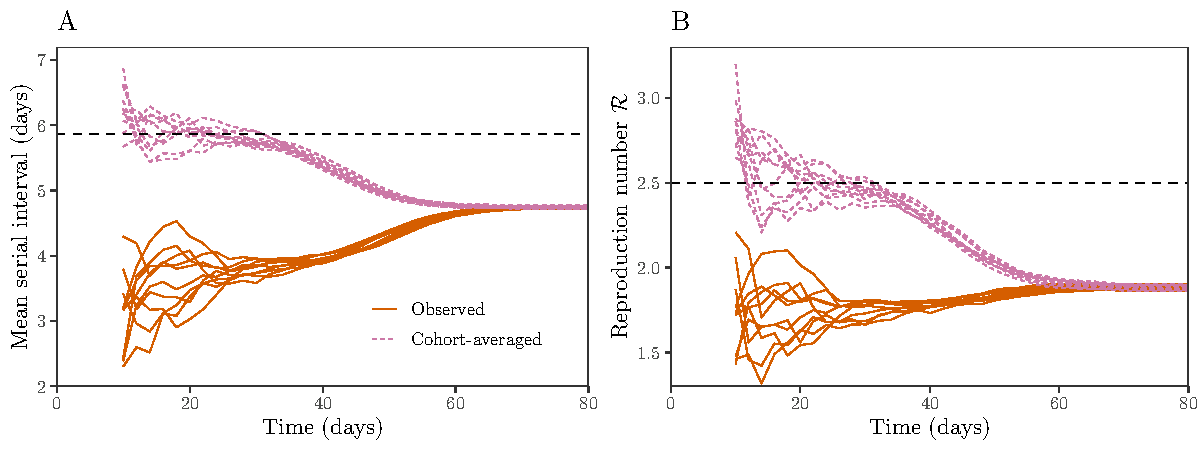
\includegraphics[width=\textwidth]{observedrR.pdf}
\caption{
\textbf{Estimates of the reproduction number from the observed serial intervals.}
A. Changes in the observed and cohort-averaged mean serial interval over time.
B. Changes in the estimate of $\mathcal R$ based on the observed and cohort-averaged mean serial interval over time.
Each line represents an independent stochastic realization.
}
\label{fig:obsrR}
\end{figure}

Now, we turn to practical issues.
When an epidemic is ongoing, the observed serial intervals are subject to right-censoring because we cannot observe a serial interval if either an infector or an infectee has not yet developed symptoms.
\fref{obsrR} demonstrates how the effect of right-censoring in the observed serial intervals translates to the underestimation of $\mathcal R$.
Notably, even if we can observe \emph{all} serial intervals across all transmission pairs after the epidemic has ended, we still underestimate the initial mean forward serial interval (\fref{obsrR}A) and therefore $\mathcal R_0$ (\fref{obsrR}) by a large amount because the observed serial-interval distribution does not account for changes in the forward serial-interval distribution.
As the mean forward serial-interval distribution decreases over time, taking the average of all observed serial intervals throughout an epidemic will underestimate the mean of the initial forward serial-interval distribution, which provides the correct linke between $r$ and $\mathcal R$.

We provide a simple, heuristic way of assessing potential biases in the estimate of $\mathcal R$ \emph{retrospctively}.
Once serial intervals have been observed after the epidemic has been sufficiently progressed, we can group observed serial intervals by their primary cohort times.
Then, we can compare how estimates of the mean serial interval and $\mathcal R$ change as we include more cohorts into the analysis (see `cohort-averaged' in \fref{obsrR}).
During the exponential growth phase, the estimates of the mean serial interval and $\mathcal R$ are consistent with the target value;
adding more data allows us to make more precise inference during this period.
However, the cohort-averaged estimates decreases rapidly soon after the exponential growth period.
This approach allows us to detect how changes in the forward serial intervals bias the estimates of $\mathcal R$.

\begin{figure}[!th]
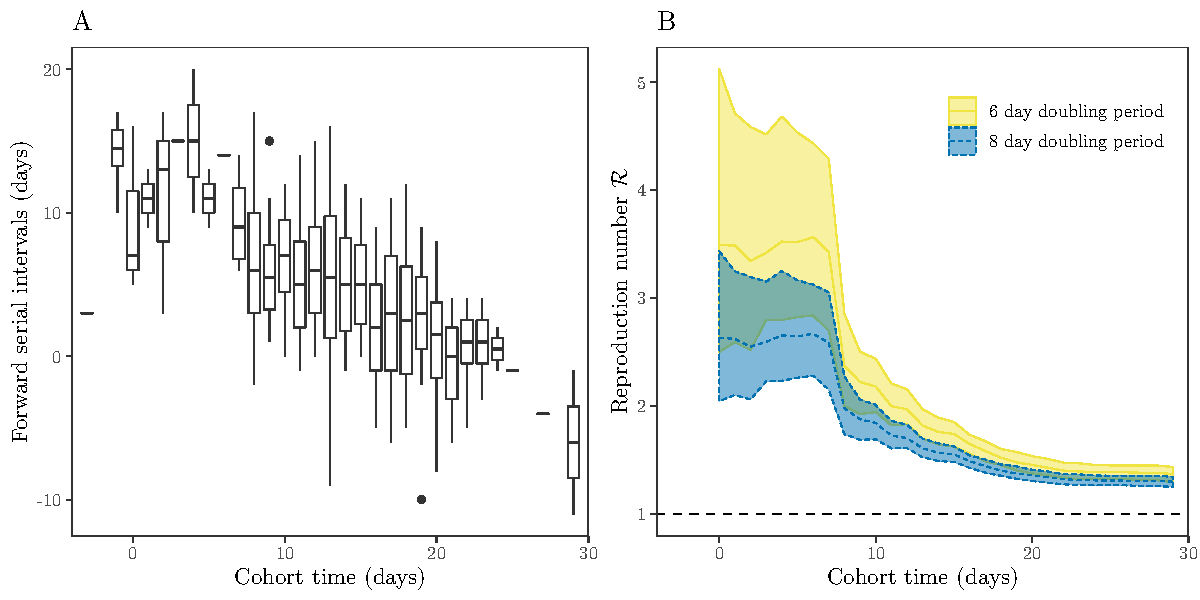
\includegraphics[width=\textwidth]{serial_analysis.pdf}
\caption{
\textbf{Observed serial intervals of COVID-19 and estimates of $\mathcal R$.}
}
\label{fig:du}
\end{figure}

Finally, we revisit serial intervals of COVID-19 collected by \cite{du2020serial} from mainland China, outside Hubei province, based on transmission events reported between January 21--February 8, 2020;
they estimated the mean serial of 3.96 days (95\% CI 3.53–4.39 days) and $\mathcal R_0$ of 1.32 (95\% CI 1.16–1.48).
\fref{du}A shows changes in the forward serial-interval distribution across cohorts.
While the observed serial intervals may be subject to right-censoring, increase in the proportion of negative serial intervals are clearly indicative of the changes in the forward serial-interval distribution.
\fref{du}B shows the cohort-averaged estimates of $\mathcal R_0$, which remain constant until day 7 and suddenly decreases.
The early cohort-averaged estimates are also consistent with earlier estimates.
This example clearly demonstrates the danger of naively averaging the observed serial intervals and calculating the reproduction number from them.

\section{Discussion}

Characterizing generation- and serial-interval distributions are critical to understanding the outset of an outbreak as they determine the time scale of disease transmission.
Generation intervals measure the time difference between infection of a transmission pair, whereas serial intervals measure the time difference between symptom onset of a transmission pair.
Due to their similar definitions, their differences have been inaccurately captured and misunderstood.

Our study demonstrate the importance of defining a cohort for studying any epidemiological time delay distributions.
Previous studies have shown that generation interval can be either measured forward or backward;
we generalize their ideas and show that these ideas can be applied to all distributions.
Changes in the backward delay distributions is particularly robust across all distributions because they depend on previous changes in cohort sizes, which, in turn, depend on incidence of infection.
Several epidemic analyses during the COVID-19 pandemic have attempted to reconstruct symptom onset or infection dates for each case from confirmed dates while assuming a constant backward delay distribution.
Although such approaches may be able to match the time scale of an epidemic, we recommend future studies to consider deconvolution approaches instead for proper reconstruction of epidemic time series.

Using cohort-based approaches, we define forward and backward serial intervals.
The forward serial-interval distribution describes the renewal process of the symptomatic individuals and therefore provides the correct link between $r$ and $\mathcal R$.
While our results support the use of serial interval distributions for calculating $\mathcal R$, 
they also reveal gaps in current approaches to characterizing serial intervals.
Previous studies have often (i) recommended using up-to-date serial intervals, (ii) assumed that the serial interval distribution remains constant, and (iii) applied serial interval distributions estimated from one location to analyzing epidemics in other locations;
however, these approaches implicitly ignore spatiotemporal variation in incidence and may therefore give systemtatically biased estimates of $\mathcal R$. 
For example, given geographical differences in the observed exponential growth rates of the COVID-19 epidemic, the forward serial interval distributions will vary across different countries.
Future studies should aim to characterize spatiotemporal variation in serial intervals and understanding the drivers of their differences.

We also show that there are multiple serial-interval distributions that correspond to the same set of generation-interval and incubation period distributions depending on their correlations;
not explicitly accounting for their correlations can bias the estimate of the intrinsic generation-interval distribution from the serial-interval distribution (see Appendix).
Furthermore, previous studies that tried to estimate the generation-interval distributions from the observed serial intervals often ignored the effect of right-censoring or differences between the backward incubation period of an infector and the forward incubation period of an infecteee.
There is currently a need for better statistical tools for teasing apart the intrinsic generation-interval distributions from the observed serial intervals.

Our study is not without limitations.
Here, we assumed that all individuals develop symptoms and that the the entire transmission process (e.g., direction of transmission, symptom onset dates, infection dates, etc.) are observable.
In practice, asymptomatic and presymptomatic transmission of COVID-19 makes measuring serial intervals difficult.
For example, symotom onset dates cannot be used as a reliable proxy for the direction of transmission as infectees may develop symptoms before their infectors.
Based on the COVID-19 paramters (Table 1), we expect roughly 3\% of infectees to develop symptoms before their infectors during the exponential growth period; 
this probability increases as epidemic progresses because backward incubation period of an infector increases.
Biases in the observed serial intervals will necessarily bias the estimates of $\mathcal R$.
Furthermore, serial intervals do not take into account asymptomatic transmission; 
not explicitly accounting for asymptomatic transmission may also  bias the estimates of $\mathcal R$.

Both generation and serial intervals are under-appreciated --- often treated as auxiliary variables for estimating $\mathcal R$ --- yet important quantities in characterizing an epidemic.
Here, we provided a theoretical basis for understanding serial intervals and show that naively using the observed serial intervals may lead to biased conclusions in studying the COVID-19 pandemic.
Concluding sentence.

\pagebreak

\section*{Appendix}

Recall that the forward serial interval can be written as:
\begin{equation}
- x_0 + \sigma + x_1
\end{equation}
Note that $x_1$ is independent of $x_0$ and $\sigma$. Then, we get:
\begin{equation}
M_{- x_0 + \sigma + x_1}(-r) = M_{- x_0 + \sigma}(-r) M_{x_1}(-r).
\end{equation}
We want to show that 
\begin{equation}
M_{- x_0 + \sigma}(-r)= \frac{M_\sigma(-r)}{M_{x_1}(-r)}
\end{equation}
for $r \geq 0$.
Note that the time between symptom onset and infection of an infectee follows the following distribution:
\begin{equation}
z(\tau) \propto \int_{\max(0, -\tau)}^\infty i(\ell - x_0) h_{\ell - x_0}(x_0, \tau+x_0) \mathrm{d} x_0.
\end{equation}
During the exponential growth phase, we have
\begin{equation}
\begin{aligned}
z_{\textrm{\tiny exp}}(\tau) &= \frac{1}{N} \int_{\max(0, -\tau)}^\infty \exp(- r x_0) h(x_0, \tau+x_0) \mathrm{d} x_0\\
% &= \frac{1}{N} \int_{0}^\infty \left[ \exp(- r x_0) k(x_0) \times \frac{h(x_0, \tau+x_0)}{k(x_0)}\right] \mathrm{d} x_0
\end{aligned}
\end{equation}
where $N$ is the normalization factor:
\begin{equation}
\begin{aligned}
N &= \int_{-\infty}^\infty \int_{\max(0, -\tau)}^\infty \exp(- r x_0) h(x_0, \tau+x_0) \mathrm{d} x_0\,\mathrm{d}\tau\\
&= \int_{0}^\infty \int_{-x_0}^\infty \exp(- r x_0) h(x_0, \tau+x_0) \mathrm{d}\tau\,\mathrm{d} x_0\\
&= \int_{0}^\infty \exp(- r x_0) k(x_0) dx_0\\
&= M_{x_1}(-r)
\end{aligned}
\end{equation}
Therefore,
\begin{equation}
\begin{aligned}
&\int_{-\infty}^{\infty} \exp(-r\tau) z_{\textrm{\tiny exp}}(\tau) \mathrm{d}\tau\\
&=\frac{1}{M_{-x_1}(-r)} \int_{-\infty}^{\infty} \exp(-r\tau) \int_{\max(0, -\tau)}^\infty \exp(- r x_0) h(x_0, \tau+x_0) \mathrm{d} x_0\, \mathrm{d}\tau
\end{aligned}
\end{equation}

Finally, we are left to prove that 
\begin{equation}
\int_0^{\infty} \exp(-r\tau) g(\tau) \mathrm{d}\tau = \int_{-\infty}^{\infty} \exp(-r\tau) \int_{\max(0, -\tau)}^\infty \exp(- r x_0) h(x_0, \tau+x_0) \mathrm{d} x_0\, \mathrm{d}\tau
\end{equation}
where $g$ is a marginal probability distribution of $h$ describing the forward generation intervals:
\begin{equation}
g(\tau) = \int_0^\infty h(x_0, \tau)  \mathrm{d} x_0.
\end{equation}
Let $a = x_0 + \tau$. Then, by change of variables, it immediately follows that
\begin{equation}
\begin{aligned}
&\int_{-\infty}^{\infty} \exp(-r\tau) \int_{\max(0, -\tau)}^\infty \exp(- r x_0) h(x_0, \tau+x_0) \mathrm{d} x_0\, \mathrm{d}\tau\\
&=\int_{0}^{\infty} \int_{0}^\infty \exp(- r a) h(x_0, a) \mathrm{d} x_0\, \mathrm{d}a\\
&=\int_{0}^{\infty} \exp(-r\tau) g(\tau) \mathrm{d}\tau
\end{aligned}
\end{equation}
Therefore, the forward serial- and generation-interval distributions give the same link between $r$ and $\mathcal R$.

\bibliography{serial}

\end{document}
